\documentclass[../231120_msquare_computational-logic.tex]{subfiles}

\begin{document}
\subsection{Introduction}

\begin{frame}{Overview}
    \begin{block}{이 세미나의 목적은...}
        \begin{enumerate}
            \ii Formal Proof의 (현실적/이론적) 필요성과 정의 \pause
            \ii ...를 알기 위한 배경(?) 지식 \pause
            \ii ...을 새내기 친화적 언어로 설명하기!
        \end{enumerate}
    \end{block}
\end{frame}

\begin{frame}{The most trustworthy types of proofs (1)}
    \begin{center}
        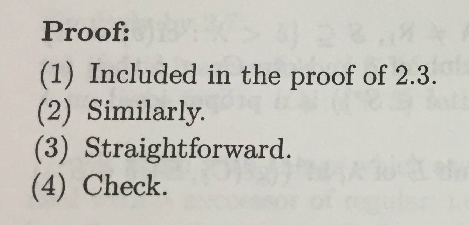
\includegraphics[width=0.7\textwidth]{./left_to_readers1.png}
    \end{center}
    \begin{center}
        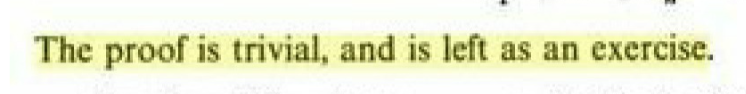
\includegraphics[width=0.8\textwidth]{./left_to_readers2.png}
    \end{center}
\end{frame}

\begin{frame}{The most trustworthy types of proofs (2)}
    \begin{center}
        {\ul{129페이지}짜리 페르마의 마지막 정리 증명}
    \end{center}
    \begin{center}
        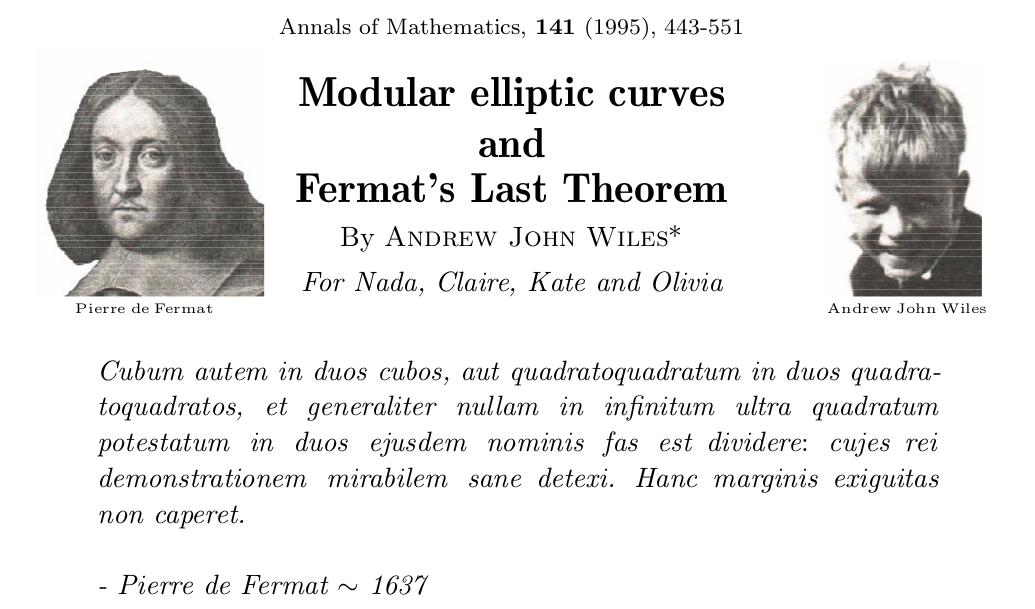
\includegraphics[width=0.7\textwidth]{./wiles_proof.png}
    \end{center}
    \pause
    \begin{center}
        이 증명을 검증하는 데에만 7+년이 걸림...
    \end{center}
\end{frame}

\begin{frame}{The most trustworthy types of proofs (3)}
    \begin{center}
        굉장히 \ul{간결하고 아름다우며} 수학자들에게\\ \ul{10년간 받아들여지고 있는}
        4색 정리의 증명
        \footnote{by Kempe, 1879}
        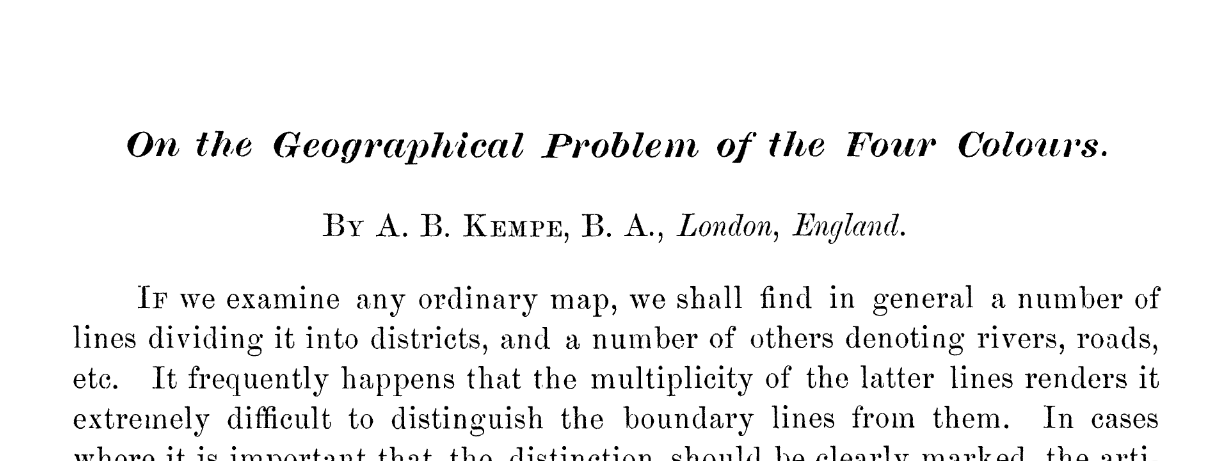
\includegraphics[width=0.8\textwidth]{./false_four_color_theorem_proof.png}
    \end{center}
\end{frame}

\begin{frame}{The most trustworthy types of proofs (3)}
    \begin{center}
        굉장히 \ul{간결하고 아름다우며} 수학자들에게\\ \ul{10년간 받아들여지고 있는}
        4색 정리의 증명
        \footnote[1]{\sout{by Kempe, 1879}}
        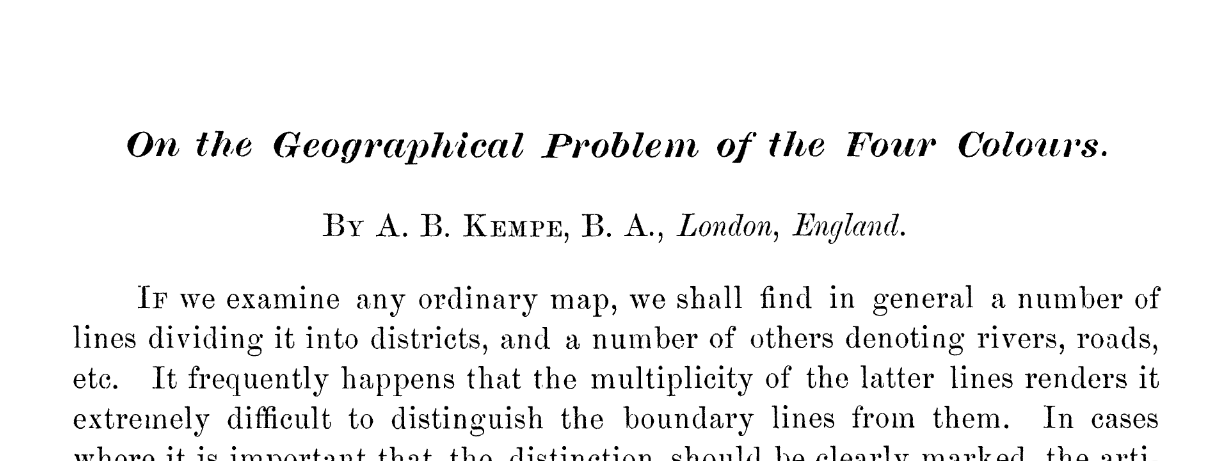
\includegraphics[width=0.8\textwidth]{./false_four_color_theorem_proof.png}
    \end{center}
    \begin{center}
        (...곧 증명의 오류가 발표될 예정인)
    \end{center}
\end{frame}

\begin{frame}{The most trustworthy types of proofs (4)}
    \begin{center}
        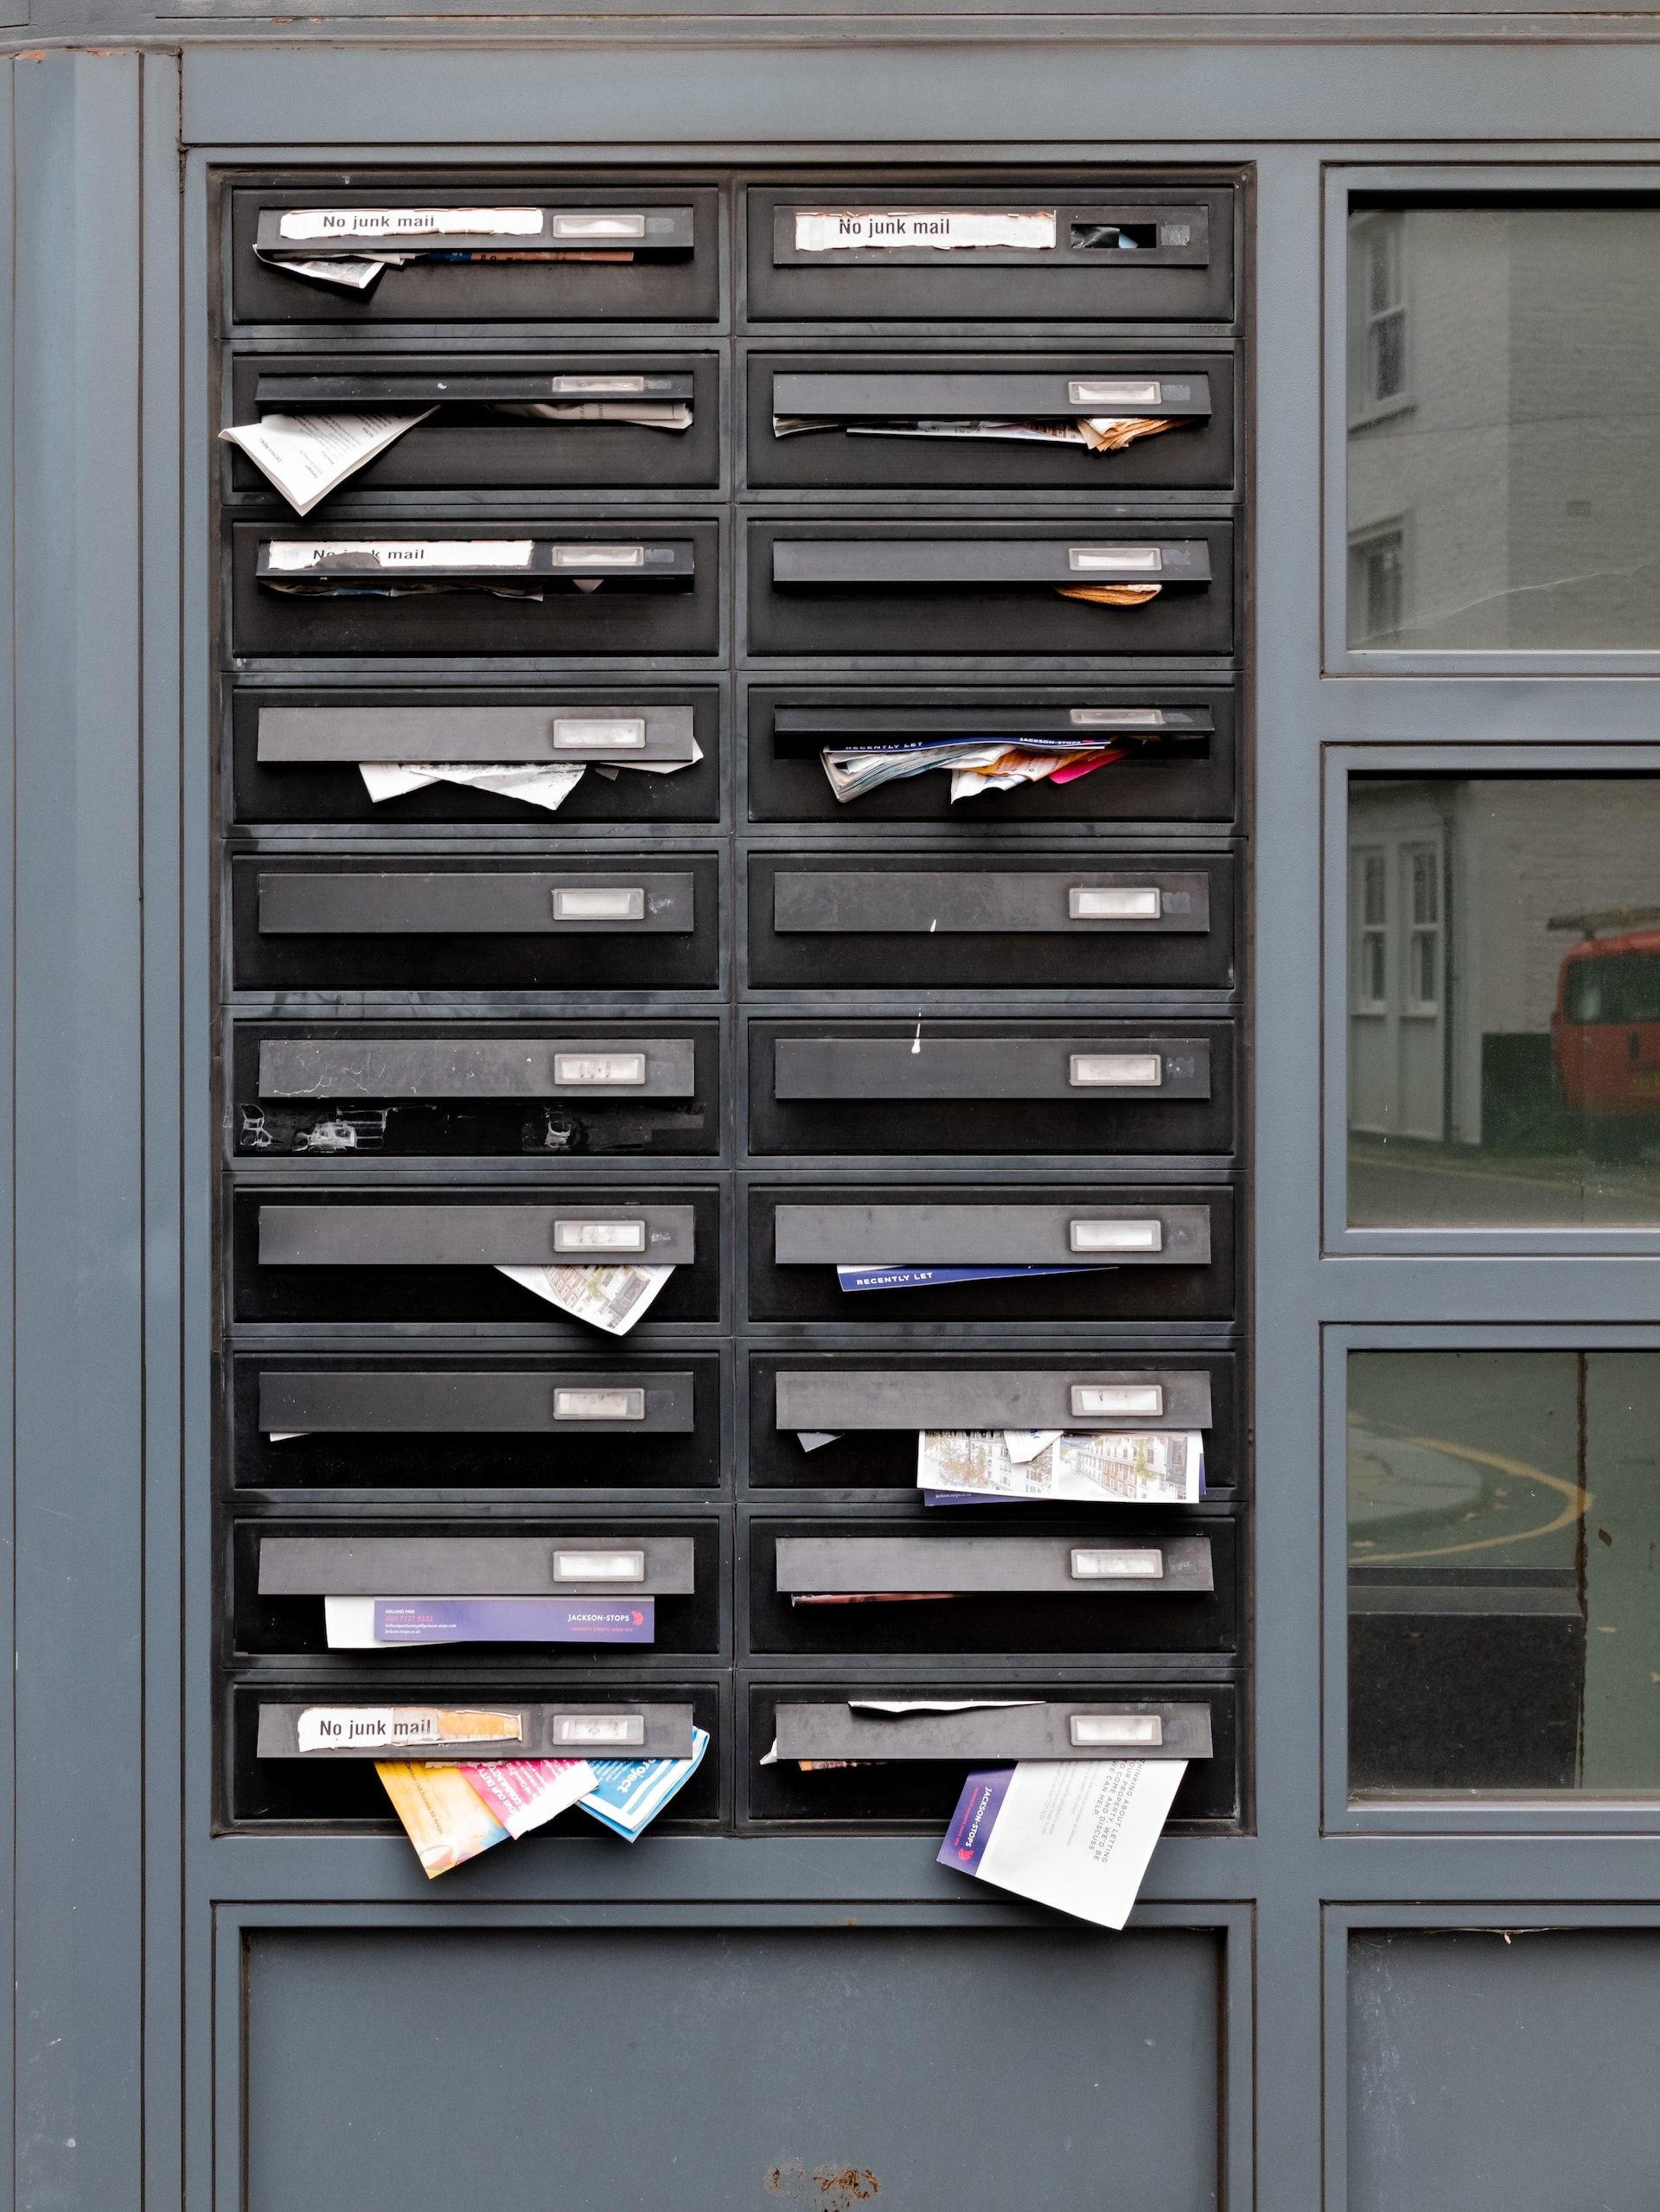
\includegraphics[width=0.4\textwidth]{./mailbox.jpg}

        매주 당신의 사무실에 도착하고 있는 리만 가설의 증명(들)...
    \end{center}
\end{frame}

\begin{frame}{Here comes the rescue!}
    \begin{exampleblock}{The Idea}
        이미 컴퓨터는 인간에게 불가능한 양의 계산을 할 수 있음...
        만약 증명을 \ul{computable object}로 끌어내린다면...?
    \end{exampleblock}
    \pause
    \begin{enumerate}
        \ii 증명의 검증을 컴퓨터에게 맡길 수 있음. \pause
        \ii 잘만 하면 증명을 생성할 수 있을지도? \pause
        \ii 수학자들 실직시킬 수 있음 \sout{\color{gray}self-unemployment} \pause
    \end{enumerate}
    \begin{alertblock}{}
        하지만 이를 위해서는 \alert{정리, 증명} 등의 \alert{명확한(수학적) \ul{정의}}가 필요!
    \end{alertblock}
\end{frame}

\begin{frame}{Overview}
    오늘 우리가 알아볼 것: \pause
    \begin{block}{}
        \begin{enumerate}
            \ii First-Order Logic
            \ii Syntax(문법)과 Semantics(의미)
            \ii Proof Theory
            \ii Theory와 Theorem(정리) \pause
            \ii Gödel's First/Second Incompleteness Theorem의 증명
                \begin{itemize}
                    \ii {\color{gray} 매우 non-rigorous함}
                        % \footnote{사실 전반적으로 굉장히 non-rigorous함}
                \end{itemize} \pause
            % \ii \alert{Automatic} Theorem Verification
            %     \begin{itemize}
            %         \ii \alert{Automatic} Theorem Proving (자동정리증명)
            %     \end{itemize}
        \end{enumerate}
    \end{block}
\end{frame}
    
\end{document}
